\documentclass[border=15pt]{standalone}
\usepackage{tikz}
\usetikzlibrary{arrows.meta}
\usepackage{fontspec}
\setmainfont{Arial}

\begin{document}

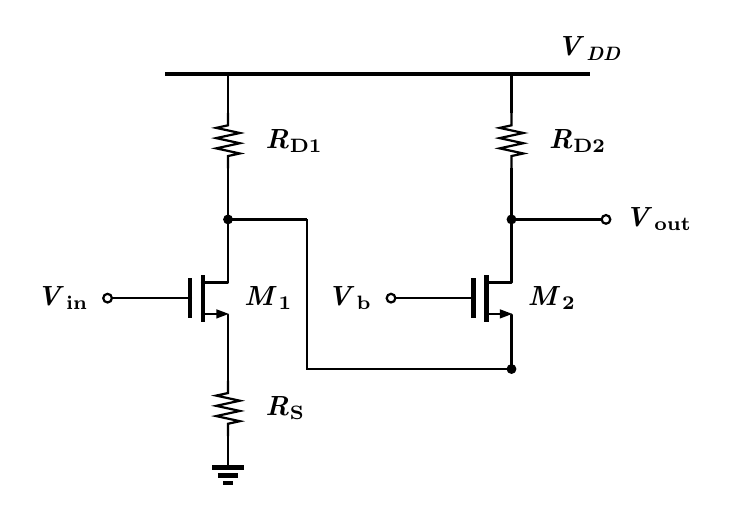
\begin{tikzpicture}[every node/.style={font=\bfseries}]
% =================================================================
% Two-Stage Circuit: CS with Source Degeneration driving CG Stage
% Optimized with latex-physics-optimize Rule 7 (XeLaTeX + Arial)
% =================================================================

% ============ ROOT: M1 (nMOS, CS Stage with Source Degeneration) ============
\begin{scope}[shift={(0, 0)}]
  \coordinate (node_M1_g) at (-0.73, 0);
  \coordinate (node_M1_d) at (0, 0.5);
  \coordinate (node_M1_s) at (0, -0.6);

  \draw[thick, line cap=round] (-0.73,0) -- (-0.47,0);
  \draw[ultra thick] (-0.48,-0.25) -- (-0.48,0.25);
  \draw[ultra thick] (-0.32,-0.3) -- (-0.32,0.3);
  \draw[thick, line cap=round, line join=round] (-0.33,0.2) -- (0,0.2) -- (0,0.5);
  \draw[-{Triangle[length=1.6mm, width=1.1mm, sep=-1.2pt]}, thick, line cap=round] (-0.33,-0.2) -- (-0.03,-0.2);
  \draw[thick, line cap=round, line join=round] (0,-0.21) -- (0,-0.6);

  \node[right=0.08cm] at (0, 0) {\normalsize \textit{M}\textsubscript{\textup{1}}};
\end{scope}

% ============ Input Terminal: Vin (IO Node on M1 Gate) ============
\begin{scope}[shift={(node_M1_g)}, xshift=-0.8cm]
  \coordinate (node_Vin_c) at (0, 0);
  \draw[thick] (0, 0) -| (node_M1_g);
  \draw[fill=white, thick] (0, 0) circle (0.055cm);
  \node[left=0.12cm] at (0, 0) {\normalsize \textit{V}\textsubscript{\textup{in}}};
\end{scope}

% ============ Source Degeneration Resistor: RS ============
\begin{scope}[shift={(node_M1_s)}, yshift=-0.8cm]
  \coordinate (node_RS_top) at (0, 0.35);
  \coordinate (node_RS_bottom) at (0, -0.35);

  \draw[thick] (0, 0.35) |- (node_M1_s);
  \draw[thick, line cap=round] (0,-0.35) -- (0,-0.195) -- (0.15,-0.1625) -- (-0.15,-0.0975) -- (0.15,-0.0325) -- (-0.15,0.0325) -- (0.15,0.0975) -- (-0.15,0.1625) -- (0,0.195) -- (0,0.35);
  \node[right=0.2cm] at (0.15, 0) {\normalsize \textit{R}\textsubscript{\textup{S}}};
\end{scope}

% ============ Ground Terminal: GND ============
\begin{scope}[shift={(node_RS_bottom)}, yshift=-0.4cm]
  \draw[thick] (0, 0) |- (node_RS_bottom);
  \draw[ultra thick] (-0.2, 0) -- (0.2, 0);
  \draw[ultra thick] (-0.13, -0.1) -- (0.13, -0.1);
  \draw[ultra thick] (-0.06, -0.2) -- (0.06, -0.2);
\end{scope}

% ============ Drain Junction 1: Black Node ============
\begin{scope}[shift={(node_M1_d)}, yshift=0.5cm]
  \coordinate (node_drain1_c) at (0, 0);
  \coordinate (node_drain1_branch_R) at (1.0cm, 0);

  \node[minimum height=0.5cm, minimum width=0.5cm, fill=white, opacity=0.01] at (0, 0) {};
  \draw[thick] (node_drain1_c) |- (node_M1_d);
  \draw[fill=black] (node_drain1_c) circle (0.055cm);
  \draw[thick] (node_drain1_c) -- (node_drain1_branch_R);
\end{scope}

% ============ Load Resistor 1: RD1 ============
\begin{scope}[shift={(node_drain1_c)}, yshift=1.0cm]
  \coordinate (node_RD1_top) at (0, 0.35);
  \coordinate (node_RD1_bottom) at (0, -0.35);

  \draw[thick] (0, -0.35) |- (node_drain1_c);
  \draw[thick, line cap=round] (0,-0.35) -- (0,-0.195) -- (0.15,-0.1625) -- (-0.15,-0.0975) -- (0.15,-0.0325) -- (-0.15,0.0325) -- (0.15,0.0975) -- (-0.15,0.1625) -- (0,0.195) -- (0,0.35);
  \node[right=0.2cm] at (0.15, 0) {\normalsize \textit{R}\textsubscript{\textup{D1}}};
\end{scope}

% ============ Power Rail: VDD ============
\begin{scope}[shift={(node_RD1_top)}, yshift=0.5cm]
  \coordinate (node_VDD_branch_R) at (4.6, 0);
  \node[minimum height=0.5cm, minimum width=5.5cm, fill=white, opacity=0.01] at (1.8, 0) {};
  \draw[thick] (0, 0) |- (node_RD1_top);
  \draw[ultra thick] (-0.8, 0) -- (4.6, 0);
  \node[above=0.05cm] at (4.6, 0) {\normalsize \textit{V}\textsubscript{\textit{DD}}};
\end{scope}

% ============ Source Junction 2: Black Node (Input of CG Stage) ============
\begin{scope}[shift={(node_drain1_branch_R)}, xshift=2.6cm, yshift=-1.9cm]
  \coordinate (node_source2_c) at (0, 0);
  \coordinate (node_source2_branch_L) at (-0.8cm, 0);

  \node[minimum height=0.5cm, minimum width=0.5cm, fill=white, opacity=0.01] at (0, 0) {};
  \draw[thick] (node_source2_c) -| (node_drain1_branch_R);
  \draw[fill=black] (node_source2_c) circle (0.055cm);
\end{scope}

% ============ STAGE 2: M2 (nMOS, Common-Gate Stage aligned with M1) ============
\begin{scope}[shift={(node_source2_c)}, yshift=0.9cm]
  \coordinate (node_M2_g) at (-0.73, 0);
  \coordinate (node_M2_d) at (0, 0.5);
  \coordinate (node_M2_s) at (0, -0.6);

  \draw[thick] (0, -0.6) |- (node_source2_c);

  \draw[thick, line cap=round] (-0.73,0) -- (-0.47,0);
  \draw[ultra thick] (-0.48,-0.25) -- (-0.48,0.25);
  \draw[ultra thick] (-0.32,-0.3) -- (-0.32,0.3);
  \draw[thick, line cap=round, line join=round] (-0.33,0.2) -- (0,0.2) -- (0,0.5);
  \draw[-{Triangle[length=1.6mm, width=1.1mm, sep=-1.2pt]}, thick, line cap=round] (-0.33,-0.2) -- (-0.03,-0.2);
  \draw[thick, line cap=round, line join=round] (0,-0.21) -- (0,-0.6);

  \node[right=0.08cm] at (0, 0) {\normalsize \textit{M}\textsubscript{\textup{2}}};
\end{scope}

% ============ Gate Bias: Vb (IO Node on M2 Gate) ============
\begin{scope}[shift={(node_M2_g)}, xshift=-0.8cm]
  \coordinate (node_Vb_c) at (0, 0);
  \draw[thick] (0, 0) -| (node_M2_g);
  \draw[fill=white, thick] (0, 0) circle (0.055cm);
  \node[left=0.12cm] at (0, 0) {\normalsize \textit{V}\textsubscript{\textup{b}}};
\end{scope}

% ============ Drain Junction 2: Black Node ============
\begin{scope}[shift={(node_M2_d)}, yshift=0.5cm]
  \coordinate (node_drain2_c) at (0, 0);
  \coordinate (node_drain2_branch_R) at (0.9cm, 0);

  \node[minimum height=0.5cm, minimum width=0.5cm, fill=white, opacity=0.01] at (0, 0) {};
  \draw[thick] (node_drain2_c) |- (node_M2_d);
  \draw[fill=black] (node_drain2_c) circle (0.055cm);
  \draw[thick] (node_drain2_c) -- (node_drain2_branch_R);
\end{scope}

% ============ Output Terminal: Vout (IO Node on M2 Drain) ============
\begin{scope}[shift={(node_drain2_branch_R)}, xshift=0.3cm]
  \coordinate (node_Vout_c) at (0, 0);
  \draw[thick] (0, 0) -| (node_drain2_branch_R);
  \draw[fill=white, thick] (0, 0) circle (0.055cm);
  \node[right=0.12cm] at (0, 0) {\normalsize \textit{V}\textsubscript{\textup{out}}};
\end{scope}

% ============ Load Resistor 2: RD2 (Aligned with RD1) ============
\begin{scope}[shift={(node_drain2_c)}, yshift=1.0cm]
  \coordinate (node_RD2_top) at (0, 0.35);
  \coordinate (node_RD2_bottom) at (0, -0.35);

  \draw[thick] (0, -0.35) |- (node_drain2_c);
  \draw[thick, line cap=round] (0,-0.35) -- (0,-0.195) -- (0.15,-0.1625) -- (-0.15,-0.0975) -- (0.15,-0.0325) -- (-0.15,0.0325) -- (0.15,0.0975) -- (-0.15,0.1625) -- (0,0.195) -- (0,0.35);
  \node[right=0.2cm] at (0.15, 0) {\normalsize \textit{R}\textsubscript{\textup{D2}}};
\end{scope}

% ============ GLOBAL CHORDS ============
% Connect Stage 2 RD2 to VDD rail flush
\draw[thick] (node_RD2_top) -- (node_RD2_top |- node_VDD_branch_R);

\end{tikzpicture}

\end{document}
